\documentclass[a4paper,11pt]{article}

% Pacotes essenciais
\usepackage[utf8]{inputenc}
\usepackage[T1]{fontenc}
\usepackage[brazil]{babel}
\usepackage{geometry}
\usepackage{graphicx}
\usepackage{float}
\usepackage{booktabs}
\usepackage{titlesec}

% Margens ajustadas para manter tudo em 2 páginas
\geometry{top=2cm, bottom=2cm, left=2cm, right=2cm}

% Formatação compacta de títulos para economizar espaço
\titleformat{\section}{\large\bfseries}{\thesection}{0.5em}{}
\titlespacing*{\section}{0pt}{10pt}{5pt}

\begin{document}

% Cabeçalho Direto
\begin{center}
    {\large \textbf{Relatório: Sistema de Rotas Urbanas - UFU campus Santa Mônica}}\\
    \textbf{Disciplina:} Estrutura de Dados 2 \quad | \quad \textbf{Prof.:} Renato Pimentel
\end{center}

% 1. Equipe e Papéis
\begin{table}[h]
    \centering
    \small
    \caption{Composição da equipe e distribuição de tarefas.}
    \begin{tabular}{ll}
        \toprule
        \textbf{Integrante} & \textbf{Papel} \\
        \midrule
        Eduardo Souza Rocha & Implementação TAD ABB \\
        Patrick Ramos Barbosa & Implementação TAD Grafo  \\
        Ítalo Lorenzo Resende Cappuzzo & Implementação do Menu Principal e Algoritmos \\
        Felipe da Conceição Silva & Arquivo de Entrada e Relatório \\
        \bottomrule
    \end{tabular}
\end{table}

\section{Definição das Estruturas de Dados}
O trabalho utiliza um \textbf{grafo não-dirigido ponderado} $G(V, A)$ com $|V|=10$ locais e $|A|=25$ conexões, conforme especificado.
\begin{itemize}
    \item \textbf{Grafo:} O grafo é \textbf{conexo}, sem vértices isolados. A representação computacional adota \textbf{Lista de Adjacências} devido à esparsidade da malha. Os pesos das arestas representam distâncias reais em metros.
    \item \textbf{Índice:} Utiliza-se \textbf{Árvore Binária de Busca (ABB)} para indexação dos locais (chave: Nome $\to$ valor: ID numérico).
\end{itemize}

\section{Algoritmos}

As funcionalidades principais do menu mapeiam-se para os seguintes algoritmos clássicos:
\begin{itemize}
    \item \textbf{Menor Rota:} Algoritmo de \textbf{Dijkstra} (para pesos não-negativos).
    \item \textbf{Árvore Geradora Mínima:} Algoritmo de \textbf{Prim} (para conexão total com custo mínimo).
\end{itemize}

\section{Listagem dos Locais}

A listagem abaixo apresenta os vértices do grafo ordenados alfabeticamente, resultado do \textbf{percurso em-ordem} na ABB.

\begin{table}[H]
    \centering
    \small
    \caption{Locais.}
    \begin{tabular}{ccl}
        \toprule
        \textbf{ID} & \textbf{Nome (Chave ABB)} & \textbf{Caracteristicas} \\
        \midrule
        2 & 1B & FACOM\\
        6 & 3Q & Livraria, Auditório\\
        4 & Biblioteca & Repositório Institucional\\
        5 & Centro\_Esportivo & Campo de futebol \\
        9 & Consultoria & ESAJUP \\
        7 & Editora\_UFU  & Editora universitária\\
        3 & LTAD  & Laboratório\\
        1 & Museu\_Mineral & Cultura \\
        0 & Reitoria & Administração central\\
        8 & RU & Provisório, PROAE\\
        \bottomrule
    \end{tabular}
\end{table}

\section{Representação Visual}

A Figura 1 exibe a estrutura topológica do grafo implementado. A Figura 2 valida a modelagem apresentando a disposição geográfica real utilizada para a coleta das distâncias (pesos).

\begin{figure}[H]
    \centering
    % Substitua pelo nome da sua imagem do grafo abstrato (bolinhas e linhas)
    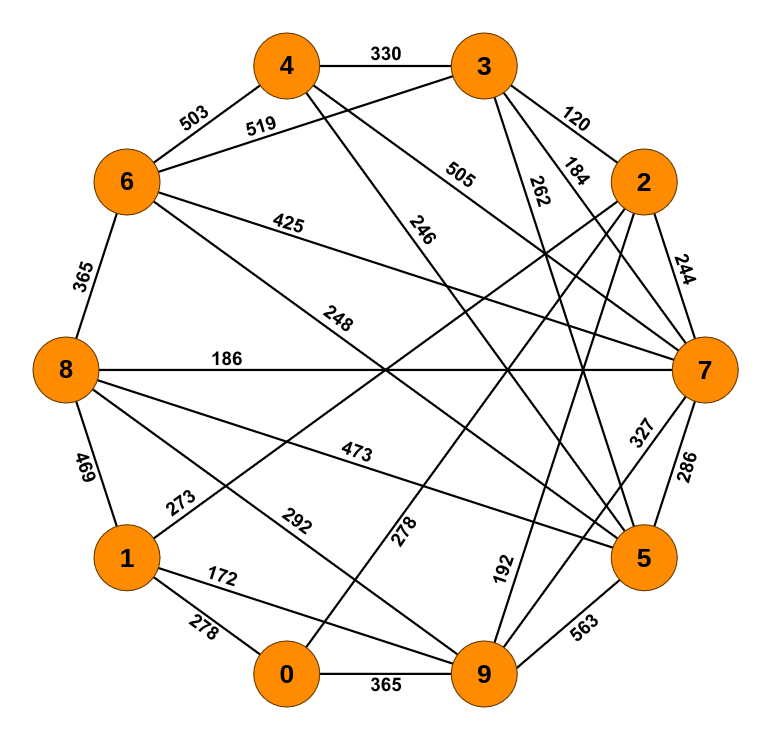
\includegraphics[width=0.7\textwidth]{grafo_abstrato.png}
    \caption{Grafo $G(V,A)$ com pesos nas arestas (distâncias em metros).}
\end{figure}

\begin{figure}[H]
    \centering
    % Substitua pelo nome da sua imagem de satélite
    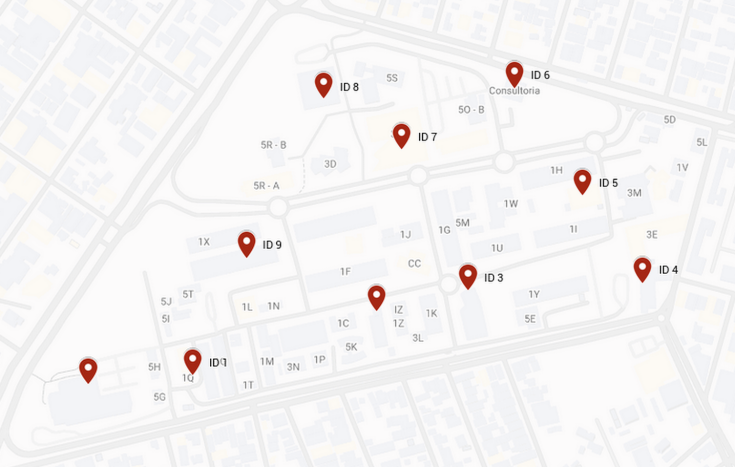
\includegraphics[width=0.65\textwidth]{ufu_mapa.png}
    \caption{Contexto geográfico: Pontos reais no Campus Santa Mônica utilizados como vértices.}
\end{figure}

\end{document}